%%%%%%%%%%%%%%%%%%%%%%%%%%%%%%%%%%%%%%%%%%%%%%%%%%%%%%%%%%%%%%%%%%%%%%%%%%%

\documentclass{standalone}

\usepackage{amsmath}
\usepackage{mathptmx}
\usepackage{pgfplots}
\usetikzlibrary{external}
\tikzexternalize{carbon14}
\pgfplotsset{compat=1.16}

%% IEEE uses Times Roman font, so we'll default to Times.
%% These three commands make up the entire times.sty package.
\renewcommand{\rmdefault}{ptm}
\renewcommand{\ttdefault}{pcr}
\normalfont\selectfont

\begin{document}

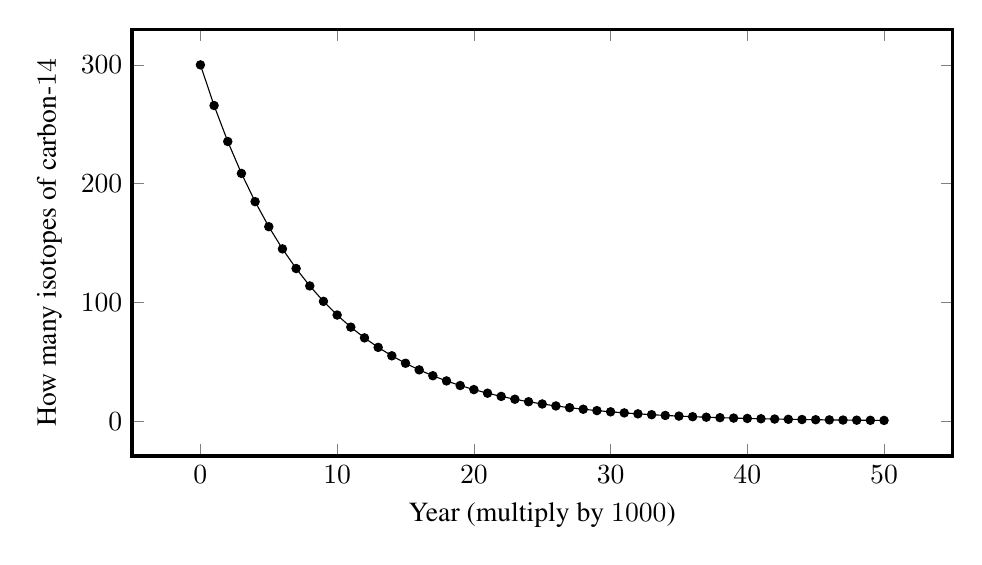
\begin{tikzpicture}
\tikzset{%%
  every mark/.append style={scale=1.0},%%
  scale=1.0%%
}
\pgfplotsset{%%
  every axis/.append style={font=\normalsize}%%
}
%%
\begin{axis}[%%
  axis line style=very thick,%%
  dotStyle/.style={mark size=1.5,black,mark color=black,mark=*},%%
  enlargelimits=true,%%
  height=7cm,%%
  width=12cm,%%
  %% x axis
  xlabel={\normalsize Year~(multiply by $1000$)},%%
  %% y axis
  ylabel={\normalsize How many isotopes of carbon-$14$},%%
  scaled y ticks=false,%%
  y tick label style=/pgf/number format/fixed%%
]
%%
%%
\addplot[dotStyle] coordinates {
  (0, 300.000000)
  (1, 265.800000)
  (2, 235.498800)
  (3, 208.651937)
  (4, 184.865616)
  (5, 163.790936)
  (6, 145.118769)
  (7, 128.575229)
  (8, 113.917653)
  (9, 100.931041)
  (10, 89.424902)
  (11, 79.230463)
  (12, 70.198190)
  (13, 62.195597)
  (14, 55.105299)
  (15, 48.823295)
  (16, 43.257439)
  (17, 38.326091)
  (18, 33.956917)
  (19, 30.085828)
  (20, 26.656044)
  (21, 23.617255)
  (22, 20.924888)
  (23, 18.539451)
  (24, 16.425953)
  (25, 14.553394)
  (26, 12.894308)
  (27, 11.424356)
  (28, 10.121980)
  (29, 8.968074)
  (30, 7.945714)
  (31, 7.039902)
  (32, 6.237353)
  (33, 5.526295)
  (34, 4.896298)
  (35, 4.338120)
  (36, 3.843574)
  (37, 3.405407)
  (38, 3.017190)
  (39, 2.673231)
  (40, 2.368482)
  (41, 2.098475)
  (42, 1.859249)
  (43, 1.647295)
  (44, 1.459503)
  (45, 1.293120)
  (46, 1.145704)
  (47, 1.015094)
  (48, 0.899373)
  (49, 0.796845)
  (50, 0.706004)
};
\end{axis}
\end{tikzpicture}

\end{document}
